%%%%%%%%%%%%%%%%%%%%%%%%%%%%%%%%%%%%%%%%%%%%%%%%%%%%%%%%%%
\begin{figure*}
\centering
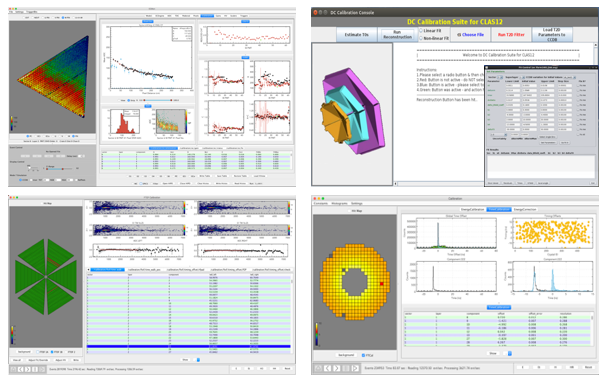
\includegraphics[width=0.9\textwidth]{pics/suites.png}
\caption{Representative subsystem calibration GUIs for ECAL~\cite{ecal-nim} (upper left),
DC~\cite{dc-nim} (upper right), FTOF~\cite{ftof-nim} (lower left),  and FT~\cite{ft-nim} (lower right).}
\label{suites}
\end{figure*}
%%%%%%%%%%%%%%%%%%%%%%%%%%%%%%%%%%%%%%%%%%%%%%%%%%%%%%%%%%%
\section{Monitoring and Calibration Suites}\label{sec:calibration}

\subsection{Framework}

A calibration framework was developed to implement visualization software tools needed for all detector
systems. Standard views were developed using the JAVA Swing application to visualize detector components and to provide callback
mechanisms necessary to display detector-component specific information.  These software tools provide
functionality for data fitting, plotting and displaying using a graphical user interface environment.

The calibration framework makes use of the other CLAS12 libraries
(the geometry and plotting packages, as well as database utilities) and provides a uniform Graphical User
Interface (GUI) for all calibration applications. The framework provides a data processing interface
and a calibration constant database interface used
for on- and off-line data analysis.

A common data streaming interface is implemented with software level abstraction that allows calibration and monitoring
code to run on variety of supported data formats used in CLAS12, including reading data in real-time from the CLAS12 DAQ system~\cite{daq-nim}.


\subsection{Calibration and Monitoring Suites}

The software programs used for the CLAS12 detector subsystem monitoring and energy and time calibrations are
Java-based suites that employ the framework discussed in Section~\ref{common-tools}.
The software tools provided by the framework facilitate the development of
detector-specific suites. Fig.~\ref{suites} shows representative views of CLAS12 subsystem calibration suites.

The calibration applications take as input raw or reconstructed data files
(from either beam data or Monte Carlo simulations) in
either EVIO or HIPO data formats.  They display the various quantities and histograms relevant to the
extraction of the calibration constants.  Each calibration suite performs fits to determine the detector subsystem
the calibration constants.  The calibration analysis parameters are saved into ASCII files
with the same structure as the tables defined in CCDB.

%%%%%%%%%%%%%%%%%%%%%%%%%%%%%%%%%%%%%%%%%%%%%%%%%%%%%%%%%%
\begin{figure*}
\centering
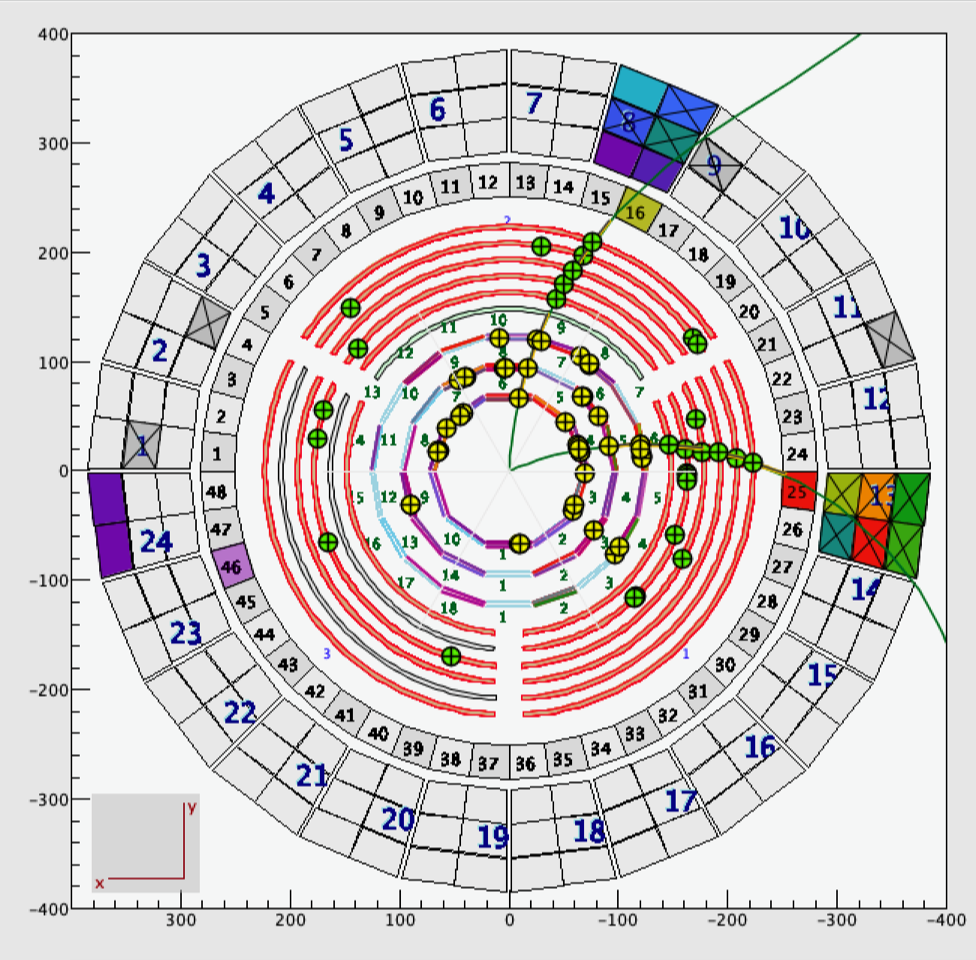
\includegraphics[width=0.4\textwidth]{pics/ced_central.png}
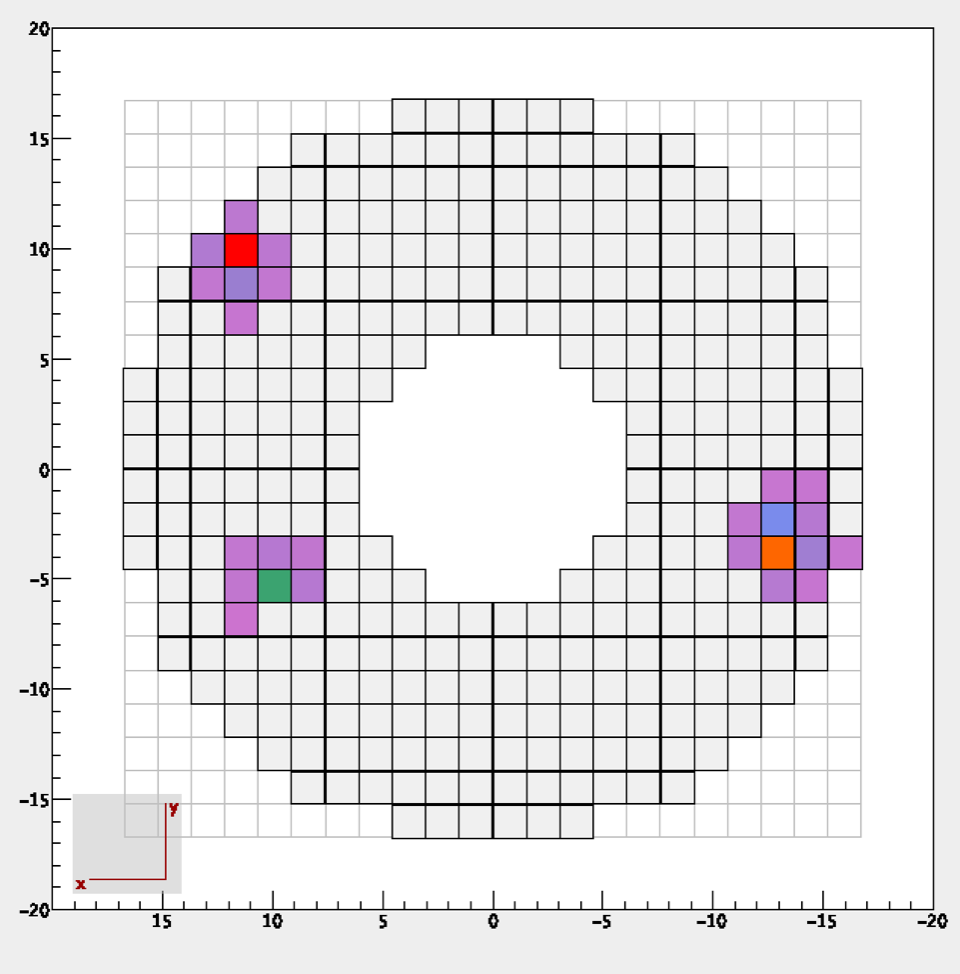
\includegraphics[width=0.39\textwidth]{pics/ced_ft.png}
\caption{ced views of the central detector (left) and of the forward tagger (right). In the central detector view, two tracks originating from the target are shown as reconstructed from the fit of the available central tracker hits in correlation with signals in the outermost detector where the color scale is representative of the recorded signal intensity. The second figure shows a front view of the Forward Tagger calorimeter for an event where three clusters were recorded.
}
\label{fig:ced}
\end{figure*}
%%%%%%%%%%%%%%%%%%%%%%%%%%%%%%%%%%%%%%%%%%%%%%%%%%%%%%%%%%%


\section{CLAS12 Event Display}\label{sec:ced}
The CLAS12 Event Display (ced) is a diagnostic graphical application for displaying CLAS12 events.
The primary element of ced is the view, i.e. a graphical representation of CLAS12 in its
entirety or a subset of detector packages.  For a given event, the primary purpose is to display the detector components that have recorded a signal, and, if available, the reconstructed tracks, providing therefore a visualization of the particle passage through the detector. In addition, ced can display information about the event such as the data banks, or information about the detector, as for example the magnetic fields. Available views are both 2- and 3-dimensional with the possibility of disabling the latter for a faster execution. An illustration of views in ced is shown in Fig.~\ref{fig:dcTracks}, where a section of the whole CLAS12 is displayed with specific focus on the forward detector: the colorful areas indicate the region where a significant magnetic field intensity is present; reconstructed tracks are shown by the orange lines. Similarly, Fig.~\ref{fig:ced} shows views of the central detector and of the forward tagger~\cite{ft-nim}. In the first, two tracks originating from the target are shown as reconstructed from the fit of the available central tracker hits in correlation with signals in the outermost detector: here, the color scale is representative of the recorded signal intensity. The second figure shows a front view of the Forward Tagger calorimeter for an event where three clusters were recorded.
ced is designed to be operated offline, reading either raw evio events or hipo events from file, or online reading events from the CLAS12 DAQ system \cite{daq-nim} to allow for real-time monitoring of the detector during data taking.
 
